\documentclass[numberedappendix]{emulateapj}
%\documentclass[iop]{emulateapj}
%apj gives the referee version/preprint2
%\usepackage[T1]{fontenc}
%\usepackage[utf8]{inputenc}
%\usepackage{graphicx}
%\usepackage{natbib}
\usepackage{amsmath}
\usepackage{amssymb}
%\usepackage{vmargin}
%\usepackage{pdfpages}
\usepackage{aas_macros}
\usepackage[normalem]{ulem}
\usepackage[usenames]{color}
\usepackage{bm}
\usepackage{cancel}
\definecolor{DarkGreen}{rgb}{0.64,0.80,0.35}
\newcommand\ALc[1]{{\color{red} \bf #1}} %Astrid
\newcommand\Ac[1]{{\color{green} \bf #1}} %% Avery
\newcommand\Pc[1]{{\color{cyan} \bf #1}} %% Phil
\newcommand\Cc[1]{{\color{blue} \bf #1}} %% Christoph
\newcommand\Ec[1]{{\color{magenta} \bf #1}} %% Ewald

\DeclareMathAlphabet\mathbfcal{OMS}{cmsy}{b}{n}
\newcommand{\calR}{\ensuremath{\bm\hat{\mathbfcal{R}}}}
\newcommand{\magcalR}{\ensuremath{\hat{\mathcal{R}}}}

\SetSymbolFont{symbols}{bold}{OMS}{cmsy}{b}{n}
%
\DeclareSymbolFont{bmisymbols}{OML}{cmm}{b}{it}
\DeclareMathSymbol{\balpha}{0}{bmisymbols}{"0B}
\DeclareMathSymbol{\bbeta}{0}{bmisymbols}{"0C}
\DeclareMathSymbol{\bgamma}{0}{bmisymbols}{"0D}
\DeclareMathSymbol{\bdelta}{0}{bmisymbols}{"0E}
\DeclareMathSymbol{\bepsilon}{0}{bmisymbols}{"0F}
\DeclareMathSymbol{\bzeta}{0}{bmisymbols}{"10}
\DeclareMathSymbol{\boldeta}{0}{bmisymbols}{"11}
\DeclareMathSymbol{\btheta}{0}{bmisymbols}{"12}
\DeclareMathSymbol{\biota}{0}{bmisymbols}{"13}
\DeclareMathSymbol{\bkappa}{0}{bmisymbols}{"14}
\DeclareMathSymbol{\blambda}{0}{bmisymbols}{"15}
\DeclareMathSymbol{\bmu}{0}{bmisymbols}{"16}
\DeclareMathSymbol{\bnu}{0}{bmisymbols}{"17}
\DeclareMathSymbol{\bxi}{0}{bmisymbols}{"18}
\DeclareMathSymbol{\bpi}{0}{bmisymbols}{"19}
\DeclareMathSymbol{\brho}{0}{bmisymbols}{"1A}
\DeclareMathSymbol{\bsigma}{0}{bmisymbols}{"1B}
\DeclareMathSymbol{\btau}{0}{bmisymbols}{"1C}
\DeclareMathSymbol{\bupsilon}{0}{bmisymbols}{"1D}
\DeclareMathSymbol{\bphi}{0}{bmisymbols}{"1E}
\DeclareMathSymbol{\bchi}{0}{bmisymbols}{"1F}
\DeclareMathSymbol{\bpsi}{0}{bmisymbols}{"20}
\DeclareMathSymbol{\bomega}{0}{bmisymbols}{"21}
\DeclareMathSymbol{\bvarepsilon}{0}{bmisymbols}{"22}
\DeclareMathSymbol{\bvartheta}{0}{bmisymbols}{"23}
\DeclareMathSymbol{\bvarpi}{0}{bmisymbols}{"24}
\DeclareMathSymbol{\bvarrho}{0}{bmisymbols}{"25}
\DeclareMathSymbol{\bvarsigma}{0}{bmisymbols}{"26}
\DeclareMathSymbol{\bvarphi}{0}{bmisymbols}{"27}


\begin{document}
\title{Probing inhomogeneous blazar heating with the Ly$\alpha$ forest}
\author{Astrid Lamberts$^1$,  Ewald Puchwein$^2$ , Philip Chang$^3$ ,Christoph Pfrommer$^4$, Avery E. Broderick$^{5,6}$ and Mohamad Shalaby$^{5,6}$}
\affil{$^1$ Theoretical Astrophysics, California Institute of Technology, Pasadena, CA, 91125, USA}
\affil{$^2$ Institute of Astronomy and Kavli Institute for Cosmology, University of Cambridge, Madingley Road, Cambridge, CB3 0HA, UK}
\affil{$^3$ Department of Physics, University of Wisconsin-Milwaukee, 1900 East Kenwood Boulevard, Milwaukee WI 53211, USA}
\affil{$^4$ Heidelberg Institute for Theoretical Studies, Schloss-Wolfsbrunnenweg 35, D-69118 Heidelberg, Germany}
\affil{$^5$ Perimeter Institute for Theoretical Physics, 31 Caroline Street North, Waterloo, ON, N2L 2Y5, Canada}
\affil{$^6$ Department of Physics and Astronomy, University of Waterloo, 200 University Avenue West, Waterloo, ON, N2L 3G1, Canada}
\email{lamberts@caltech.edu}
\begin{abstract}

\end{abstract}
\keywords{}
\section{Introduction}
%% The intergalactic medium constitutes the bulk of the baryons forming the cosmic web \citep{1996Natur.380..603B} as well as the reservoir of baryons available for the formation of galaxies and clusters \citep{1997ApJ...489....7R}. Observations of metal-enriched gas link its evolution to the formation of galaxies and stars (see e.g. \citet{2009A&A...493..409S,2010MNRAS.407.2063W}). Therefore, the thermal history of the IGM plays a central role in determining the development of structure in the visible universe.

%% The temperature of the IGM is mostly set by photoionization of hydrogen and helium, competing with adiabatic cooling. As a result, the universe is slowly cooling once reionization is completed. The IGM temperature is expected to increase with density because denser regions experience a lower amount of adiabatic cooling, as well as more recombination-induced photoheating. Gas in the IGM that has not been shock heated provides a lower envelope to the temperature-density distribution.  Observations of Lyman $\alpha$ absorption lines with $4\leqslant z \leqslant 2$ show that lower column density gas exhibits the lowest line widths, which is commonly interpreted as an indication that lower density gas is colder than high density gas \citep{1997ApJ...484..672K,2000MNRAS.318..817S,2000ApJ...534...41R,2012ApJ...757L..30R}. A temporary flattening of the slope of the inferred temperature-density relation around $z\sim 3$ indicates an additional source of heating at that redshift.

%% The latter is expected due to He\,\textsc{II} reionization \citep[e.g.][]{2007MNRAS.380.1369T,2009ApJ...694..842M,2013MNRAS.435.3169C,2014arXiv1410.1531P}. Observations suggest that the tail end of He\,\textsc{II} reionization occurred between $z \simeq 3.2$ and 2.7 \citep{2001Sci...293.1112K,2014ApJ...784...42S}. However, the bulk of He\,\textsc{II} has likely ionized earlier, potentially as early as $z\ge 4$ \citep{2014arXiv1405.7405W}.  Its patchiness is probably related to the rarity of ionizing sources and the inhomogeneity of the IGM.  Including full radiative transfer, simulations show enhanced scatter in the temperature-density distribution around $z=3$ \citep{2009ApJ...694..842M}. Whether reionization may result in an inverted temperature-density distribution \citep{2012MNRAS.423....7M} is not firmly established yet \citep{2013MNRAS.435.3169C}. 

%% On top of that, recent measurements found that underdense regions may be warmer than predicted \citep{2009MNRAS.399L..39V,2008MNRAS.386.1131B}, as well as to exhibit unexpectedly high temperatures at $z<2$ \citep{2014MNRAS.441.1916B}, which is harder to explain solely by ionization of He\,\textsc{II}. Although an inverted temperature-density relation in underdense regions has not been firmly established yet \citep{2014MNRAS.438.2499B}, these observations suggest that the thermal history of the IGM may be more complex than initially assumed.

%% \citet{2012ApJ...752...22B} recently suggested a complementary heating mechanism, through TeV blazars. TeV blazars are active galactic nuclei (AGN) emitting very high energy gamma rays ($E\ge100$~GeV). They belong to the radio-loud subgroup of AGN, with the relativistic jet being pointed towards us. About 50 of these sources have been significantly discovered so far (http://tevcat.uchicago.edu/) by ground based Cerenkov telescopes such as MAGIC, H.E.S.S. and VERITAS. Those pointed observations have only skimmed the surface of a much larger population that manifest themselves as hard-spectra gamma-ray blazars as observed with the space-based \textit{Fermi}-LAT telescope \citep{2014ApJ...790..137B}. 

%% The universe is mainly opaque to very high energy gamma rays; they interact with the extragalactic background light (EBL) producing electron/positron pairs \citep{1967PhRv..155.1408G,1992ApJ...390L..49S}. It is commonly assumed that the electron/positron pairs inverse Compton scatter photons of the cosmic microwave background, resulting in a distribution of photons with energies between $0.1$ and $100$ GeV. Such an emission component towards TeV blazars has not been observed so far \citep{2010A&A...524A..77A}, despite extended searches \citep{2014A&A...562A.145H}. One solution would be pair deflection due to the intergalactic magnetic field, thus lowering the surface brightness of the formed pair halo at GeV energies \citep{2013A&ARv..21...62D,2012ApJ...747L..14V,2011ApJ...733L..21D}. 

%% However, the cascaded GeV emission would still contribute to the extragalactic gamma-ray background (EGRB). \textit{Fermi}-LAT was able to resolve more sources than its predecessor EGRET, thereby limiting the isotropic component of the unresolved EGRB and severely constraining the redshift evolution of hard blazars in the presence of inverse Compton cascades \citep[e.g.,][]{Vent:10,Murase:2012,Inoue:2012}. As a result of these, it is now well established that in this picture, the co-moving number density of gamma-ray blazars, and by extension the TeV blazars, must either be constant or decreasing with redshift \citep{Knei-Mann:08,Vent:10,Abazajian:2011,Inoue:2012}.  This lies in stark contrast to other classes of AGNs specifically, and all other tracers of the cosmological history of accretion onto galactic halos generally (e.g., star formation).  Furthermore, after careful modeling of gamma-ray and X-ray survey selection effects there appears to be no evidence for a significantly different evolution of blazars in comparison to their radio-loud analogues such as radio galaxies \citep{Giommi:2012,Giommi:2013}. Together this casts doubt on the inverse Compton cascade picture and provides circumstantial evidence that pair beams instead transfer their energy directly to the IGM through plasma instabilities \citep{2012ApJ...752...22B, 2012ApJ...758..102S, 2013ApJ...777...49S,2014ApJ...797..110C}. This naturally explains the EGRB with a blazar population that exhibits a redshift evolution in agreement with that of quasars \citep{2014ApJ...790..137B,2014ApJ...796...12B}.

%% The pairs constitute a dilute, ultrarelativistic beam, which is subject to several plasma instabilities, from which the ``oblique'' instability \citep{PhysRevE.70.046401} is the most powerful. Assuming its efficiency in the linear regime extends to the non-linear regime, \citet{2012ApJ...752...23C} show it is responsible for increasing the temperature of the IGM by almost a factor 10 in low density regions. While this assumption is still debated (see \citet{2013ApJ...770...54M,2014ApJ...787...49S} but also \citet{2013ApJ...777...49S,2012ApJ...758..102S,2014ApJ...797..110C}), throughout all this paper we assume plasma instabilities are the dominant mechanism for cooling of the pair beams.

%% Including TeV blazar heating in the thermal history of the IGM, \citet{2012ApJ...752...23C} were able to reproduce the inverted temperature-density relation for low density regions. \citet{2012ApJ...752...24P} found that TeV blazar heating  is capable of creating a redshift dependent entropy floor in clusters and galaxies, thus suppressing the formation of dwarf galaxies after the peak of blazar activity at redshift $z\simeq2$ and potentially providing an explanation to the ``missing satellite problem'' and the ``missing void dwarf problem'' \citep{2010AdAst2010E...8K}. Implementing uniform blazar heating, i.e. with a redshift-dependent but spatially homogeneous energy deposition rate per unit volume, in a cosmological hydrodynamical simulation of galaxy formation, \citet{2012MNRAS.423..149P} find excellent agreement with the one and two-point statistics of the Lyman $\alpha$ forest, which is the main observational tracer of low density regions in the universe.

%% However, the low thermal broadening of certain Lyman $\alpha$ lines indicates the presence of cold gas at $z =2.4$ \citep{2012ApJ...757L..30R}, which suggests TeV blazar heating does not uniformly heat the whole universe. It is natural to expect a larger TeV flux close to higher density regions where visible structures form. Conversely, in large underdense regions, far from massive black holes, heating is probably much lower. The goal of this paper is to go beyond the hypothesis of uniform heating and to link TeV blazar heating to the underlying clustered density field and take into account the bias of sources. This will lead to a more heterogeneous heating pattern and account for unheated regions while keeping the overall impact of blazar heating.

%% Self-consistently studying the evolution of the IGM from first principles involves modeling both the formation and evolution of galaxies at the largest scales of the universe. As this is still far beyond reach of current computers, we have determined a filter function which relates the heating fluctuations to the dark matter (DM) structure similarly to \citet{2007MNRAS.376.1680P,2005ApJ...626....1B,2014PhRvD..89h3010P}. Based on the hierarchical structure formation in a $\Lambda$CDM universe, it naturally selects the relevant length scales for TeV blazar heating ($\S$2). We have implemented it in large scale cosmological simulations ($\S$3) in order to focus on the equation of state and thermal evolution of the IGM ($\S$4). We then discuss how inhomogeneous heating could reconcile different observations ($\S$5) and conclude ($\S$6).
%% EBL. Despite careful studies that aim at constraining it, there remain uncertainties in the star formation history of the universe as well as its metallicity and dust contents \citep[see, e.g.][]{2008A&A...487..837F,2006ApJ...648..774S}. Following \citet{2012ApJ...752...23C} we use a prescription


\section{Cosmological simulations}

Our simulations are very similar to the simulations presented in Paper I and are performed at higher resolution. In this section we remind the reader of their relevant characteristics. 

We perform our simulations with \textsc{GADGET-3}, which is and upgraded version of \textsc{GADGET-2} \citep{2005MNRAS.364.1105}.  It is based on a Smoothed Particle Hydrodynamics (SPH) scheme and solves the gravitational evolution of gas and dark matter with a TREE-PM N-body method.  The equations of hydrodynamics are solved with an entropy conserving scheme based on \citep{2002MNRAS.333..649S}.   Our simulations are based on the cosmological parameters based on  the \textit{Planck} data combined with lensing, \textit{WMAP} and high multipole measurements \citep{2014A&A...571A..16P}: $\Omega_M = 0.305$, $\Omega_{\lambda} = 0.694$, $\Omega_B = 0.0481$, $h = 0.679$, $\sigma_8 = 0.827$ and $n_s$ = 0.962.  These values are slightly updated with respect to the simulations presented in \citep{2012MNRAS.423..149P,2015ApJ...811...19L}. \ALc{[I don't expect this to have any influence, is that correct?]}

We start our simulations based on initial conditions evolved up to redshift $z=110$ and stop our simulations at $z=1.74$, beyond which observational date is sparse \ALc{[I'm considering to go to lower z and look if we can solve the ``photon underproduction crisis''].}. As this work focusses on the IGM, we use a simplified model for star formation, where gas particles with  density $\delta_{\mathrm{gas}}\geq 1000$ and T $\leq 10^5$ are directly converted into stars \citep{2004MNRAS.354..684V}. While this can yield inaccurate galaxy properties, it does not affect the low-density IGM and significantly speeds up the simulations. We also neglect direct black hole feedback.


\ALc{[Paragraph about UV  background and related stuff here]}

We perform a set of three simulations, one without any blazar heating, one with uniform blazar heating and one with inhomogeneous blazar heating.  The uniform blazar heating model is identical to the ``intermediate heating'' model presented in \citet{2012MNRAS.423..149P}.  Our inhomogeneous model has the same total amount of energy injected by blazars while accounting for regions receiving more or less heating according to their proximity to heating sources. The model is fully described in Paper I  and is based on an analytic formalism relating the distribution of the heating rate to the underlying dark matter distribution. It results in the  filtering function shown on Fig.~\ref{fig:window}, which  removes small scale fluctuations and enhances fluctuations beyond $\simeq 10$ h$^{-1}$ Mpc at $z=4$ and $\simeq 40$ h$^{-1}$ Mcp at $z=2$.  The shape and redshift evolution of the  window function is set by the mean free path of the VHEGR combined with the bias of the heating sources.  While we presented two models in Paper I, with galaxy bias and quasar bias, in this work we focus on the model with quasar bias, which is probably more representative of the bias of TeV blazars.  

\begin{figure}[h]
\centering
 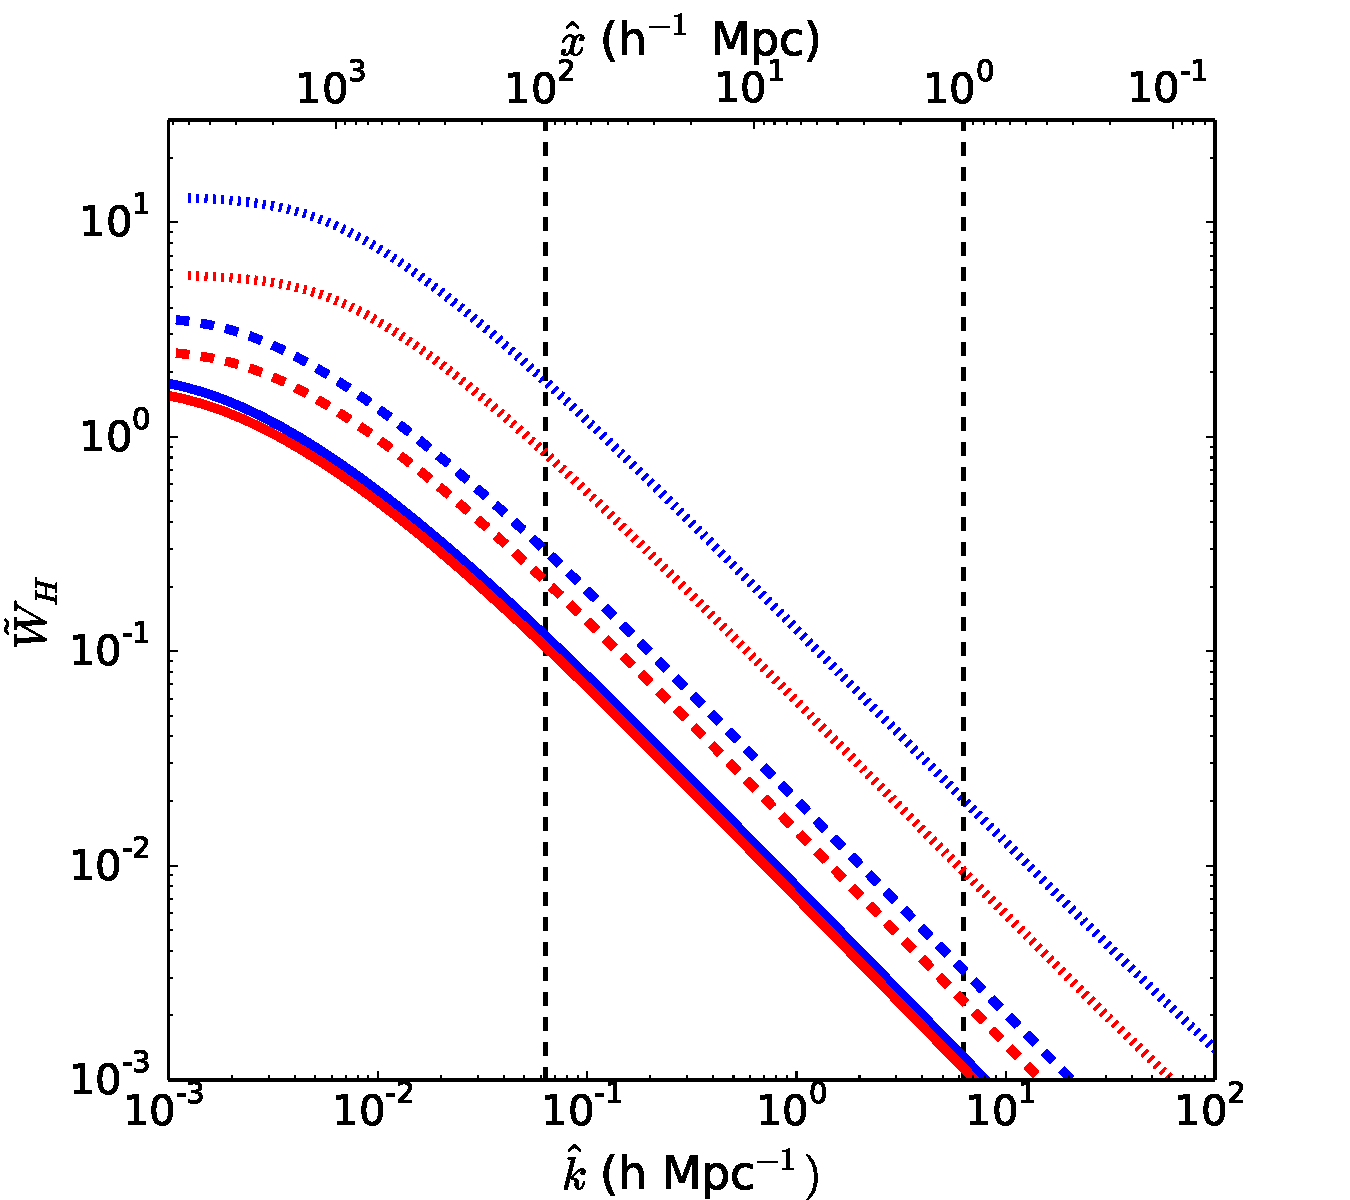
\includegraphics[width = .45\textwidth ]{window_gal_qso}

\caption{Window function for TeV blazar heating from $z=1$ (solid lines), $z=2$ (dashed lines) and $z=4$ (dotted lines) for the galaxy bias model (red) and the quasar bias model (blue).  The vertical dashed lines indicate the minimal and maximal comoving wavenumber modeled in the simulation. \ALc{Placeholder, will remove galaxy bias and add more appropriate redshift lines}}
\label{fig:window}
\end{figure}

Because of the typical length scale of the heating rate fluctuations, our simulation have a comoving sidelength of  a $100$ h$^{-1}$ Mpc.  Tests in Paper I showed that this is a sufficiently large size to properly sample the full range of temperature fluctuations. \ALc{Discuss resolution here}



%We use $N= 2\times 512^3$ particles, which gives a mass of $m_\mathrm{gas}=3.8\times10^{6} h^{-1} M_{\odot}$ and $m_\mathrm{DM}=1.8\times 10^{7} h^{-1} M_{\odot}$ for baryonic and dark matter particles, respectively. We used a comoving gravitational softening length of 7.8 $h^{-1}$ kpc. We checked that the resolution has a barely discernible impact on the results of our simulations by performing test simulations with a comoving side length of 50 $h^{-1}$ Mpc at different resolutions, up to $2\times 512^3$. The spread of the temperature in the low density regions increases with increasing resolution. However, this effect is approaching saturation at a resolution of $N=2\times 256^3$. We find less than $4\%$ difference in the median temperature and less than $10\%$ difference in its root mean square in low density regions between $N=2\times 256^3$ and $2\times 512^3$ simulations, indicating that our chosen resolution is sufficient to accurately capture the temperature-density distribution. 

% Photoheating is set by ionization equilibrium of H, He\,\textsc{I} and He\,\textsc{II} in the presence of an external UV field, which is parameterized according to \citet{2009ApJ...703.1416F}. As our version of the \textsc{GADGET-3} code assumes ionization equilibrium when computing photoheating rates, the heating is rather inefficient during reionization where this assumption is not well satisfied \citep[see e.g.][]{2014arXiv1410.1531P}. Following \citet{2012MNRAS.423..149P} we thus include the equivalent heat input by hand at redshift $z=10$. Our simulation does not include radiative transfer effects on the photoionization of He\,\textsc{II}.



\section{Comparison with observations}
\subsection{Post-processing the simulations}
\begin{itemize}
\item Global flow , potential caveats
\item Details about subdividing LOS in chunks for VPFIT
\end{itemize}

\begin{figure*}[h]
\centering
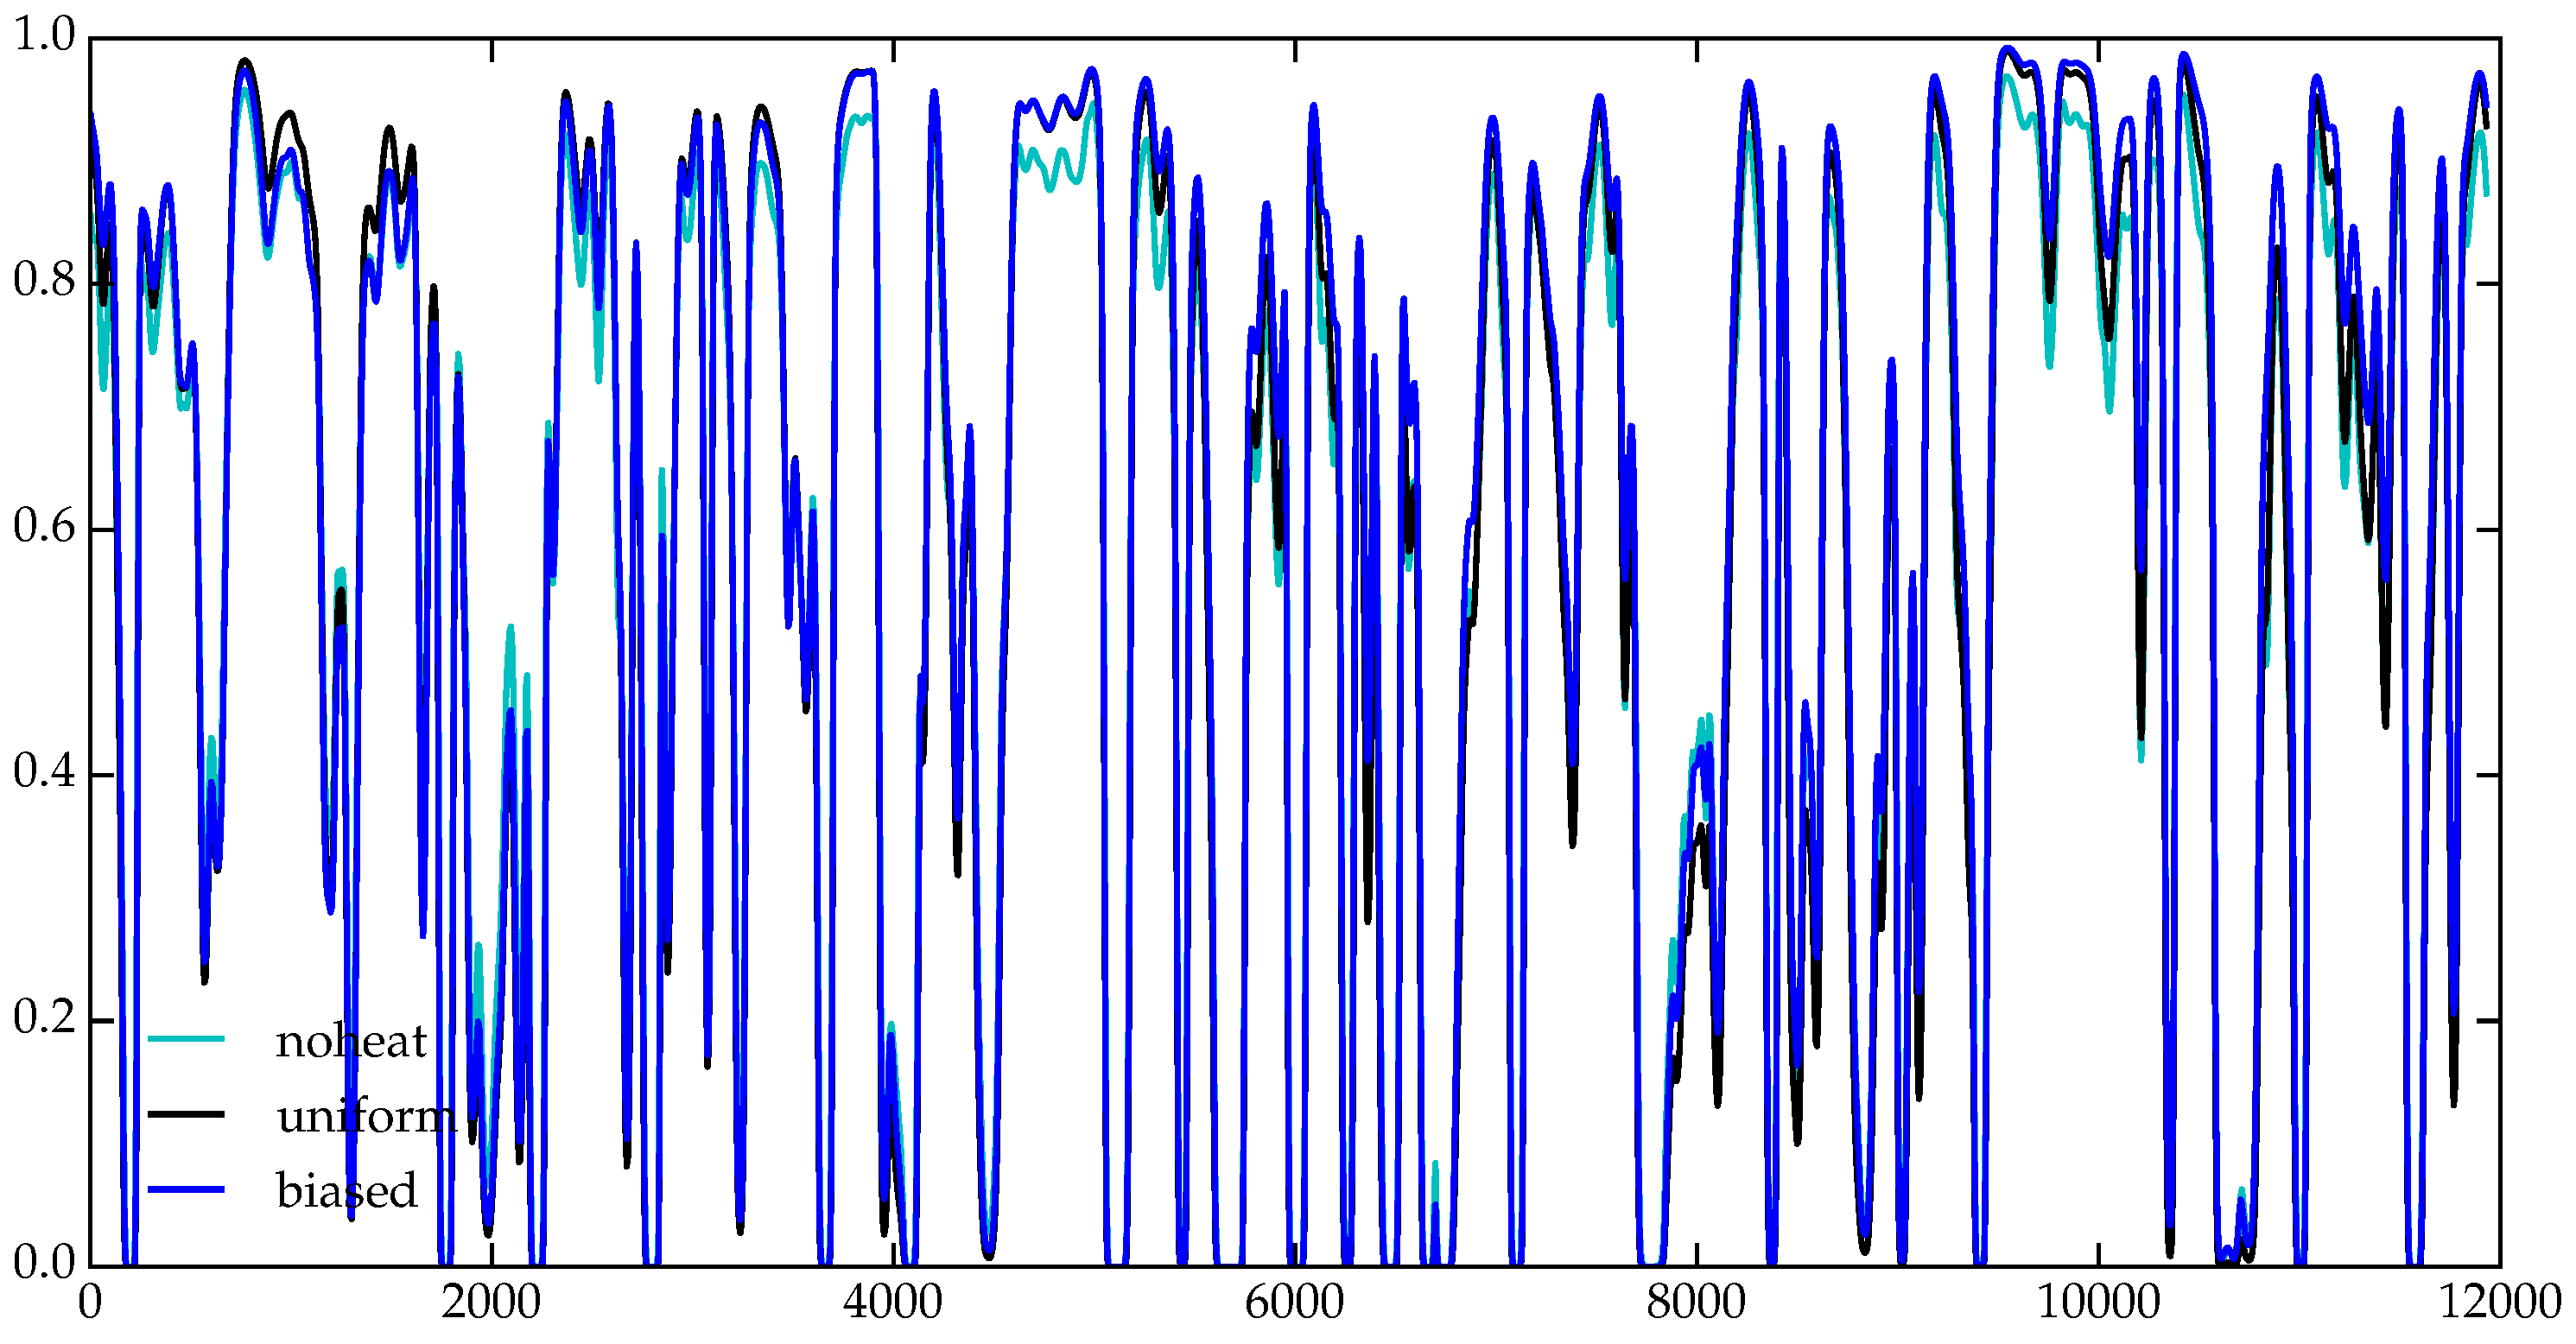
\includegraphics[width = .8\textwidth ]{lines_z2_2}
\caption{Ly$\alpha$ absorption spectrum at $z=2.2$ in the three models. \ALc{[Placeholder, will be improved]}}
\label{fig:bias}
\end{figure*}

\subsection{Ly$\alpha$ forest statistics}


\begin{figure}[h]
\centering
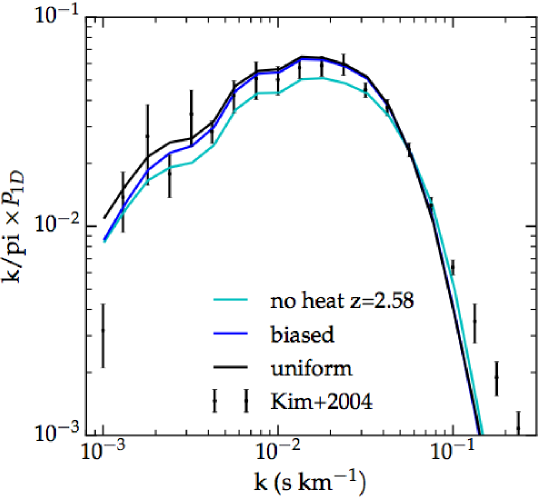
\includegraphics[width = .45\textwidth ]{powerspec}
\caption{ Power spectrum at different redshifts compare with observations \ALc{[Placeholder, will be improved]}}
\label{fig:powespec}
\end{figure}

\begin{figure*}[h]
\centering
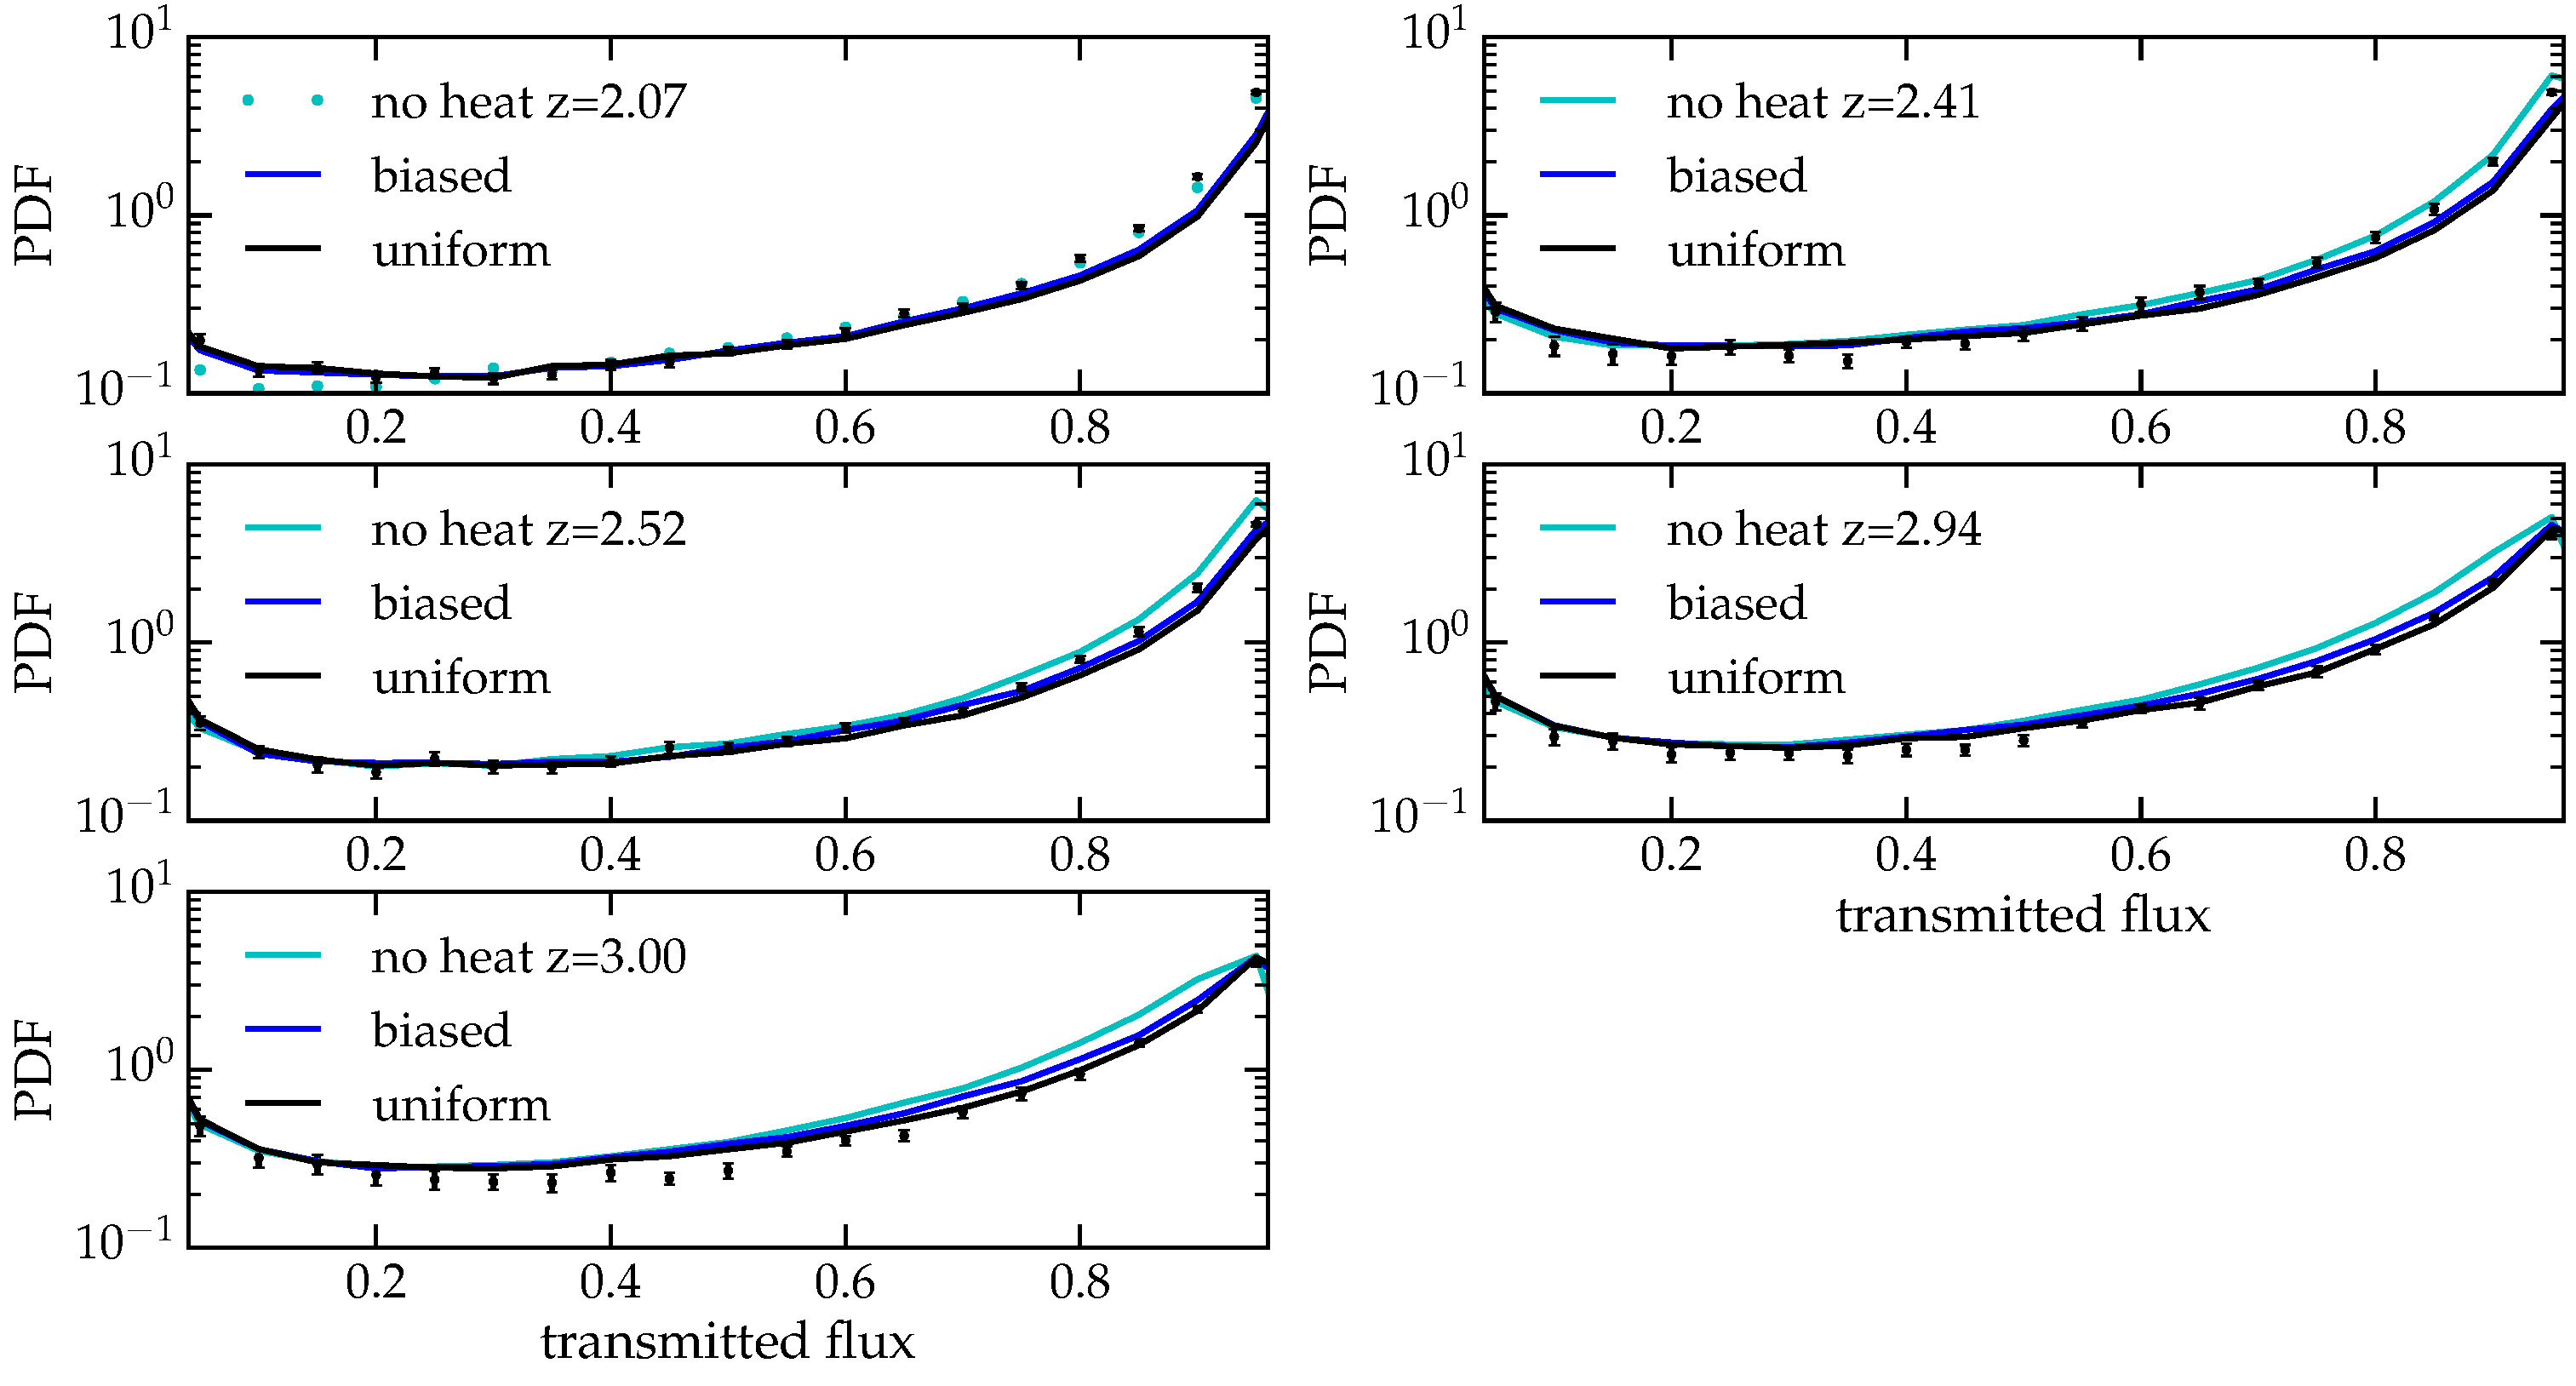
\includegraphics[width = .9\textwidth ]{flux_PDF}
\caption{Flux PDF at different redshifts compare with observations \ALc{[Placeholder, will be improved]}}
\label{fig:fluxPDF}
\end{figure*}

\subsection{Thermal state of the IGM}
\begin{enumerate}
\item Compare with Rorai 2016
\item Maybe compare with low-z results
\item Rudie and other b-Nh distributions
\end{enumerate}
\begin{figure}
\centering
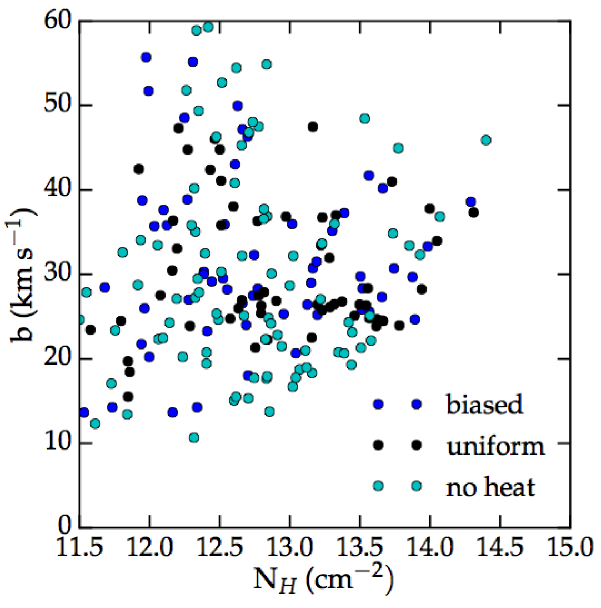
\includegraphics[width = .45\textwidth ]{b_Nh}
\caption{ Column density - Doppler with distribution in the different models \ALc{[Placeholder, will be improved]}}
\label{fig:b_Nh}
\end{figure}



\section{Discussion}

\section{Conclusions}

\begin{acknowledgements}
%% AL and PC are supported by the UWM Research Growth Initiative, the NASA ATP
%% program through NASA grant NNX13AH43G, and NSF grant AST-1255469.
%% A.E.B.~and M.S.~receive financial support from the Perimeter
%% Institute for Theoretical Physics and the Natural Sciences and
%% Engineering Research Council of Canada through a Discovery Grant.
%% Research at Perimeter Institute is supported by the Government of
%% Canada through Industry Canada and by the Province of Ontario through
%% the Ministry of Research and Innovation.
%% C.P.~gratefully acknowledges
%% financial support of the Klaus Tschira Foundation. E.P. acknowledges support by the ERC grant ``The Emergence of Structure during the epoch of Reionization''.
%% The authors acknowledge the Texas Advanced Computing Center (TACC) at The University of Texas at Austin and the NASA Advanced Supercomputing Division for providing HPC resources that have contributed to the research results reported within this paper. The authors thank S. Furlanetto, A. Loeb and M. Heahnelt for fruitful discussions. 
\end{acknowledgements}

\bibliographystyle{apj}
\bibliography{biblio_total}
\end{document}
